\subsection[Cos'è Java]{Cos'è Java}

\pgfdeclareimage[width=3cm]{javalogo}{img/javalogo.png}
\begin{frame}{Java}
 
  \begin{center}
    \pgfuseimage{javalogo}
  \end{center}
  
\end{frame}

\begin{frame}{Cos'è Java (I)}
  
  Java Language Specification (788 pagg.)\footnote{\url{https://docs.oracle.com/javase/specs/jls/se8/jls8.pdf}}
  \begin{quote}
   «The Java$^{\textregistered}$  programming  language is a general-purpose, [...] 
    class-based,  object-oriented  language.»
  \end{quote}

  Java è:
  \begin{itemize}
    \item un \textbf{linguaggio} (grammatica, vocabolario, sintassi, ecc.);
    \item linguaggio di \textbf{programmazione};
    \item general-purpose (vs domain-specific, e.g. \textit{SQL});
    \item orientato agli \textbf{oggetti} (attributi, metodi);
    \item class-based (\textbf{classe}, ereditarietà);
  \end{itemize}

\end{frame}

\begin{frame}{Cos'è Java (II)}
  
  Altre caratteristiche di Java:
  \begin{itemize}
    \item \textbf{imperativo} (vs. funzionale vs. logico);
  \end{itemize}
\end{frame}

{
  \setbeamercolor{background canvas}{bg=}
  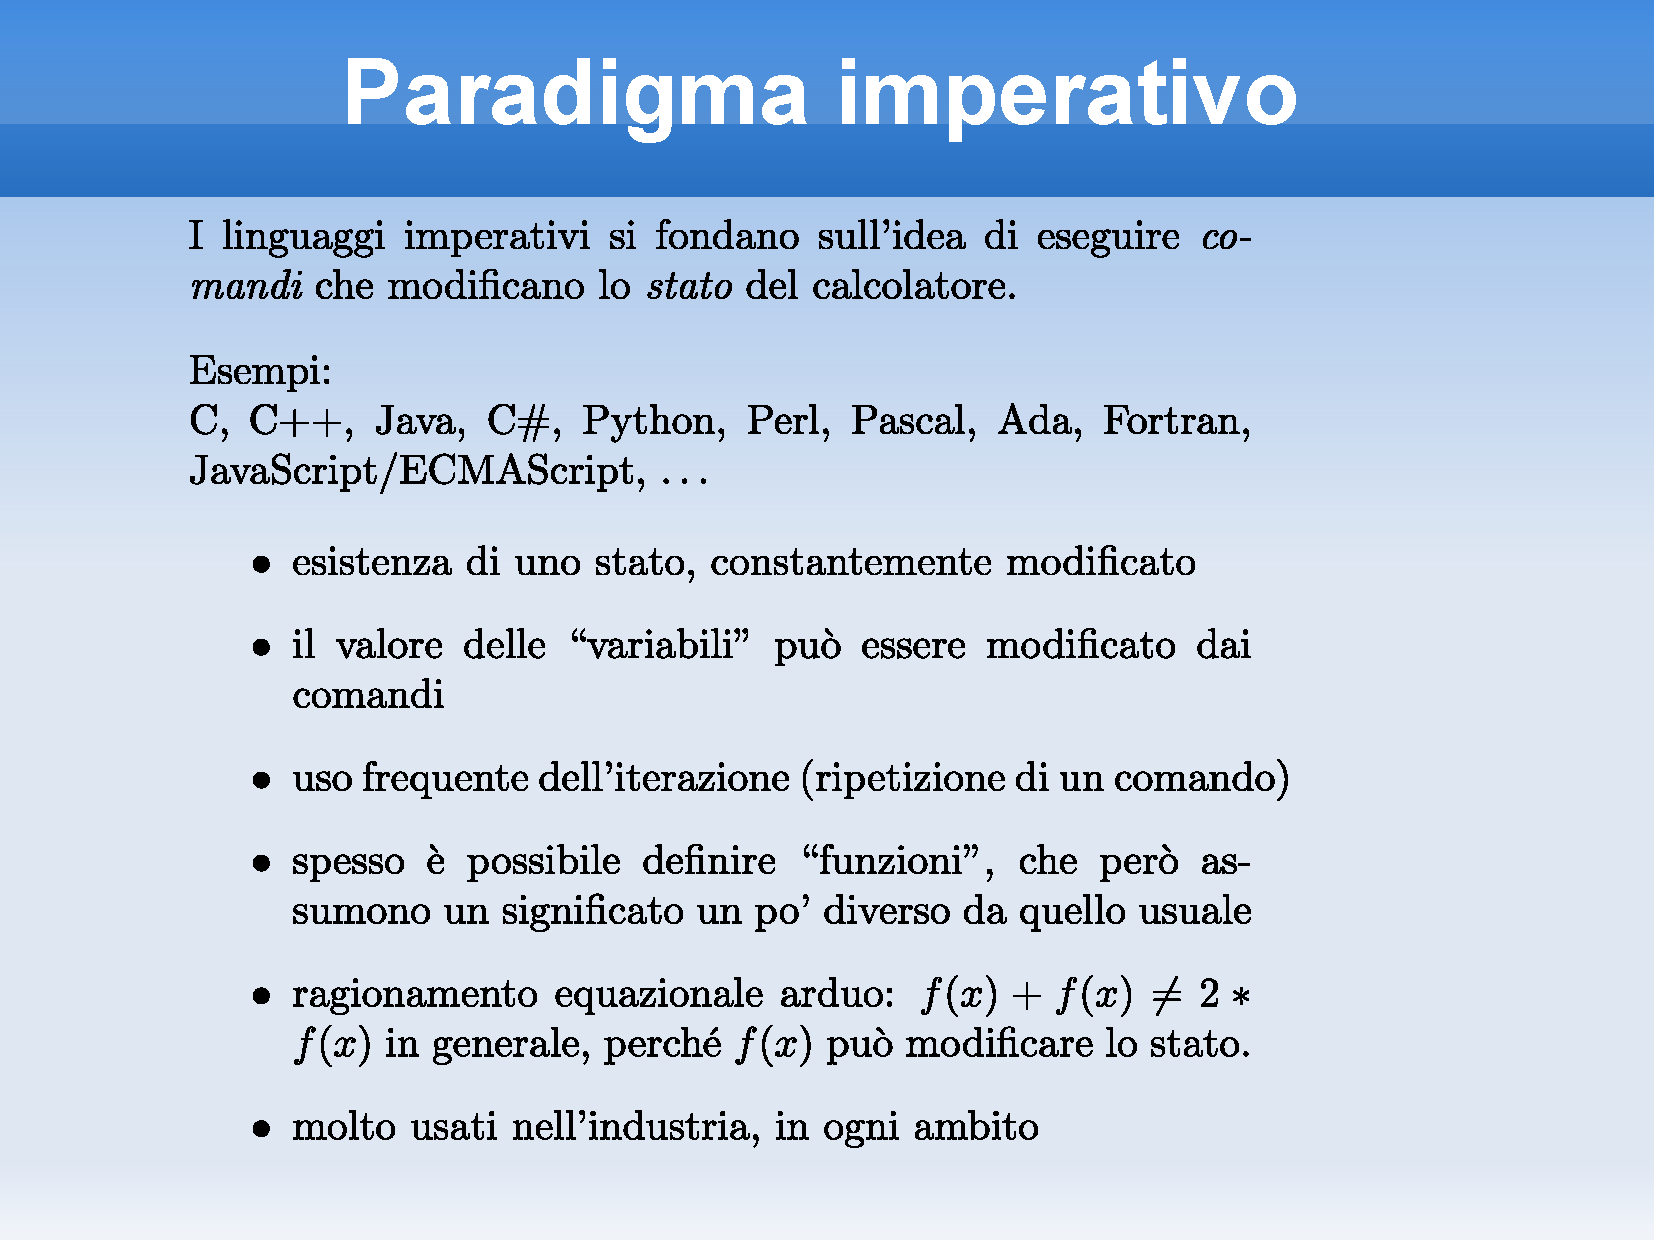
\includepdf[pages={1}]{img/imperativo.pdf}
}

\begin{frame}{Cos'è Java (II)}
  
  Altre caratteristiche di Java:
  \begin{itemize}
    \item \textbf{imperativo} (vs. funzionale vs. logico);
    \item \textbf{compilato} (vs. interpretato);
    \item \textbf{fortemente tipizzato}, \emph{strongly typed} (vs. debolmente tipizzato)
    \item Molto usato in svariati ambiti;
    \item ...
  \end{itemize}
\end{frame}

\subsection[Altri linguaggi]{Altri linguaggi}

\begin{frame}{Altri linguaggi}

  Esistono moltissimi altri linguaggi:
  \begin{itemize}
    \item ad es. linguaggi di markup (e.g. HTML, XML, TeX)
    \item altri linguaggi \textbf{di programmazione}: C, C++, python,
  go, Scala, Prolog, Perl, $\dots$

  \end{itemize}
\end{frame}

\pgfdeclareimage[width=0.5\paperwidth]{hello_c}{img/hello_c.png}
\begin{frame}{Altri linguaggi (II)}
  \textbf{C}:
  \begin{center}
    \pgfuseimage{hello_c}
  \end{center}
\end{frame}

\pgfdeclareimage[width=0.5\paperwidth]{hello_py}{img/hello_py.png}
\begin{frame}{Altri linguaggi (III)}
  \textbf{Python}:
  \begin{center}
    \pgfuseimage{hello_py}
  \end{center}
\end{frame}

\pgfdeclareimage[width=0.5\paperwidth]{hello_java}{img/hello_java.png}
\begin{frame}{Altri linguaggi (IV)}
  \textbf{Java}:
  \begin{center}
    \pgfuseimage{hello_java}
  \end{center}
\end{frame}


\pgfdeclareimage[width=0.5\paperwidth]{hello_c_exe}{img/hello_c_exe.png}
\begin{frame}{Altri linguaggi (V)}
  \textbf{C}:
  \begin{center}
    \pgfuseimage{hello_c_exe}
  \end{center}
\end{frame}

\pgfdeclareimage[width=0.5\paperwidth]{hello_py_exe}{img/hello_py_exe.png}
\begin{frame}{Altri linguaggi (VI)}
  \textbf{Python}:
  \begin{center}
    \pgfuseimage{hello_py_exe}
  \end{center}
\end{frame}

\pgfdeclareimage[width=0.5\paperwidth]{hello_java_exe}{img/hello_java_exe.png}
\begin{frame}{Altri linguaggi (VII)}
  \textbf{Java}:
  \begin{center}
    \pgfuseimage{hello_java_exe}
  \end{center}
\end{frame}

\pgfdeclareimage[width=0.5\paperwidth]{hello_c_comp}{img/hello_c_comp.png}
\begin{frame}{Altri linguaggi (VIII)}
  \textbf{C (bynary)}:
  \begin{center}
    \pgfuseimage{hello_c_comp}
  \end{center}
\end{frame}

\pgfdeclareimage[width=0.75\paperwidth]{hello_java_comp}{img/hello_java_comp.png}
\begin{frame}{Altri linguaggi (IX)}
  \textbf{Java (bytecode)}:
  \begin{center}
    \pgfuseimage{hello_java_comp}
  \end{center}
\end{frame}

\begin{frame}{Pseudocodice}

  Per esprimere un algoritmo senza adottare una sintassi legata ad un particolare
  linguaggio si usa lo \textbf{pseudocodice}:
    \begin{algorithmic}[1]
      
      \State $sum \gets 0$
      \For{$i \gets 1$ to $N$}
	\For{$j \gets 0$ to $i$}
	  \If{$i \mod 2 = 0$}
	    \State $sum \gets sum + 1$ 
	  \EndIf
	\EndFor
      \EndFor
    \end{algorithmic}

\end{frame}

\begin{frame}{Pseudocodice (II)}

  Per esprimere un algoritmo senza adottare una sintassi legata ad un particolare
  linguaggio si usa lo \textbf{pseudocodice}:
  
  (Esempio di dichiarazione di funzioni)
  \begin{algorithmic}[H]
    \Function{InsertionSort}{Array $x$}
      \For{$i \gets \len{A}$}
	\State $value \gets A[i]$
	\State $j \gets i - 1$
	\While{$j \geq 0$ $\wedge$ $A[j] > value$}
	  \State $A[j + 1] \gets A[j]$
	  \State $j \gets j-1$
	\EndWhile
      \EndFor
    \EndFunction
  \end{algorithmic}

\end{frame}